\externaldocument{Introduction.tex}
\externaldocument{Experimental_Apparatus.tex}
\externaldocument{Results.tex}
\externaldocument{Analysis.tex}
\externaldocument{EIC_Jets.tex}
\externaldocument{Checks_and_Systematics.tex}
\externaldocument{Discussion.tex}

\chapter{First Photon-Tagged Fragmentation Results in \pPb}

\section{Fully Subtracted Correlation Functions}
\label{sec:decaybkgsubtraction}
The final $ \gammaiso$-hadron correlations are reported in $\zt$  bins for each trigger-photon $\pt$~bin, where $\zt$~is the ratio of the associated hadron, $\pt^\mathrm{h}$, to isolated photon transverse momentum, $\zt = \pt^{\mathrm{h}}/\pt^{\gammaiso}$. The fully subtracted azimuthal correlations as a function of $ \Delta\varphi$, the azimuthal angle between the photon and the hadron, are shown in Fig.~\ref{fig:GH_Correlations} for pp and \pPb~data. With the measured \gammaiso~ constraining the parton kinematics, the distribution of away-side associated hadrons with momentum fraction \zt~represents the fragmentation function of the parton. The systematic uncertainties are discussed in detail in Chapter~\ref{sec:systematics}.

 \begin{figure*}
     \centering
     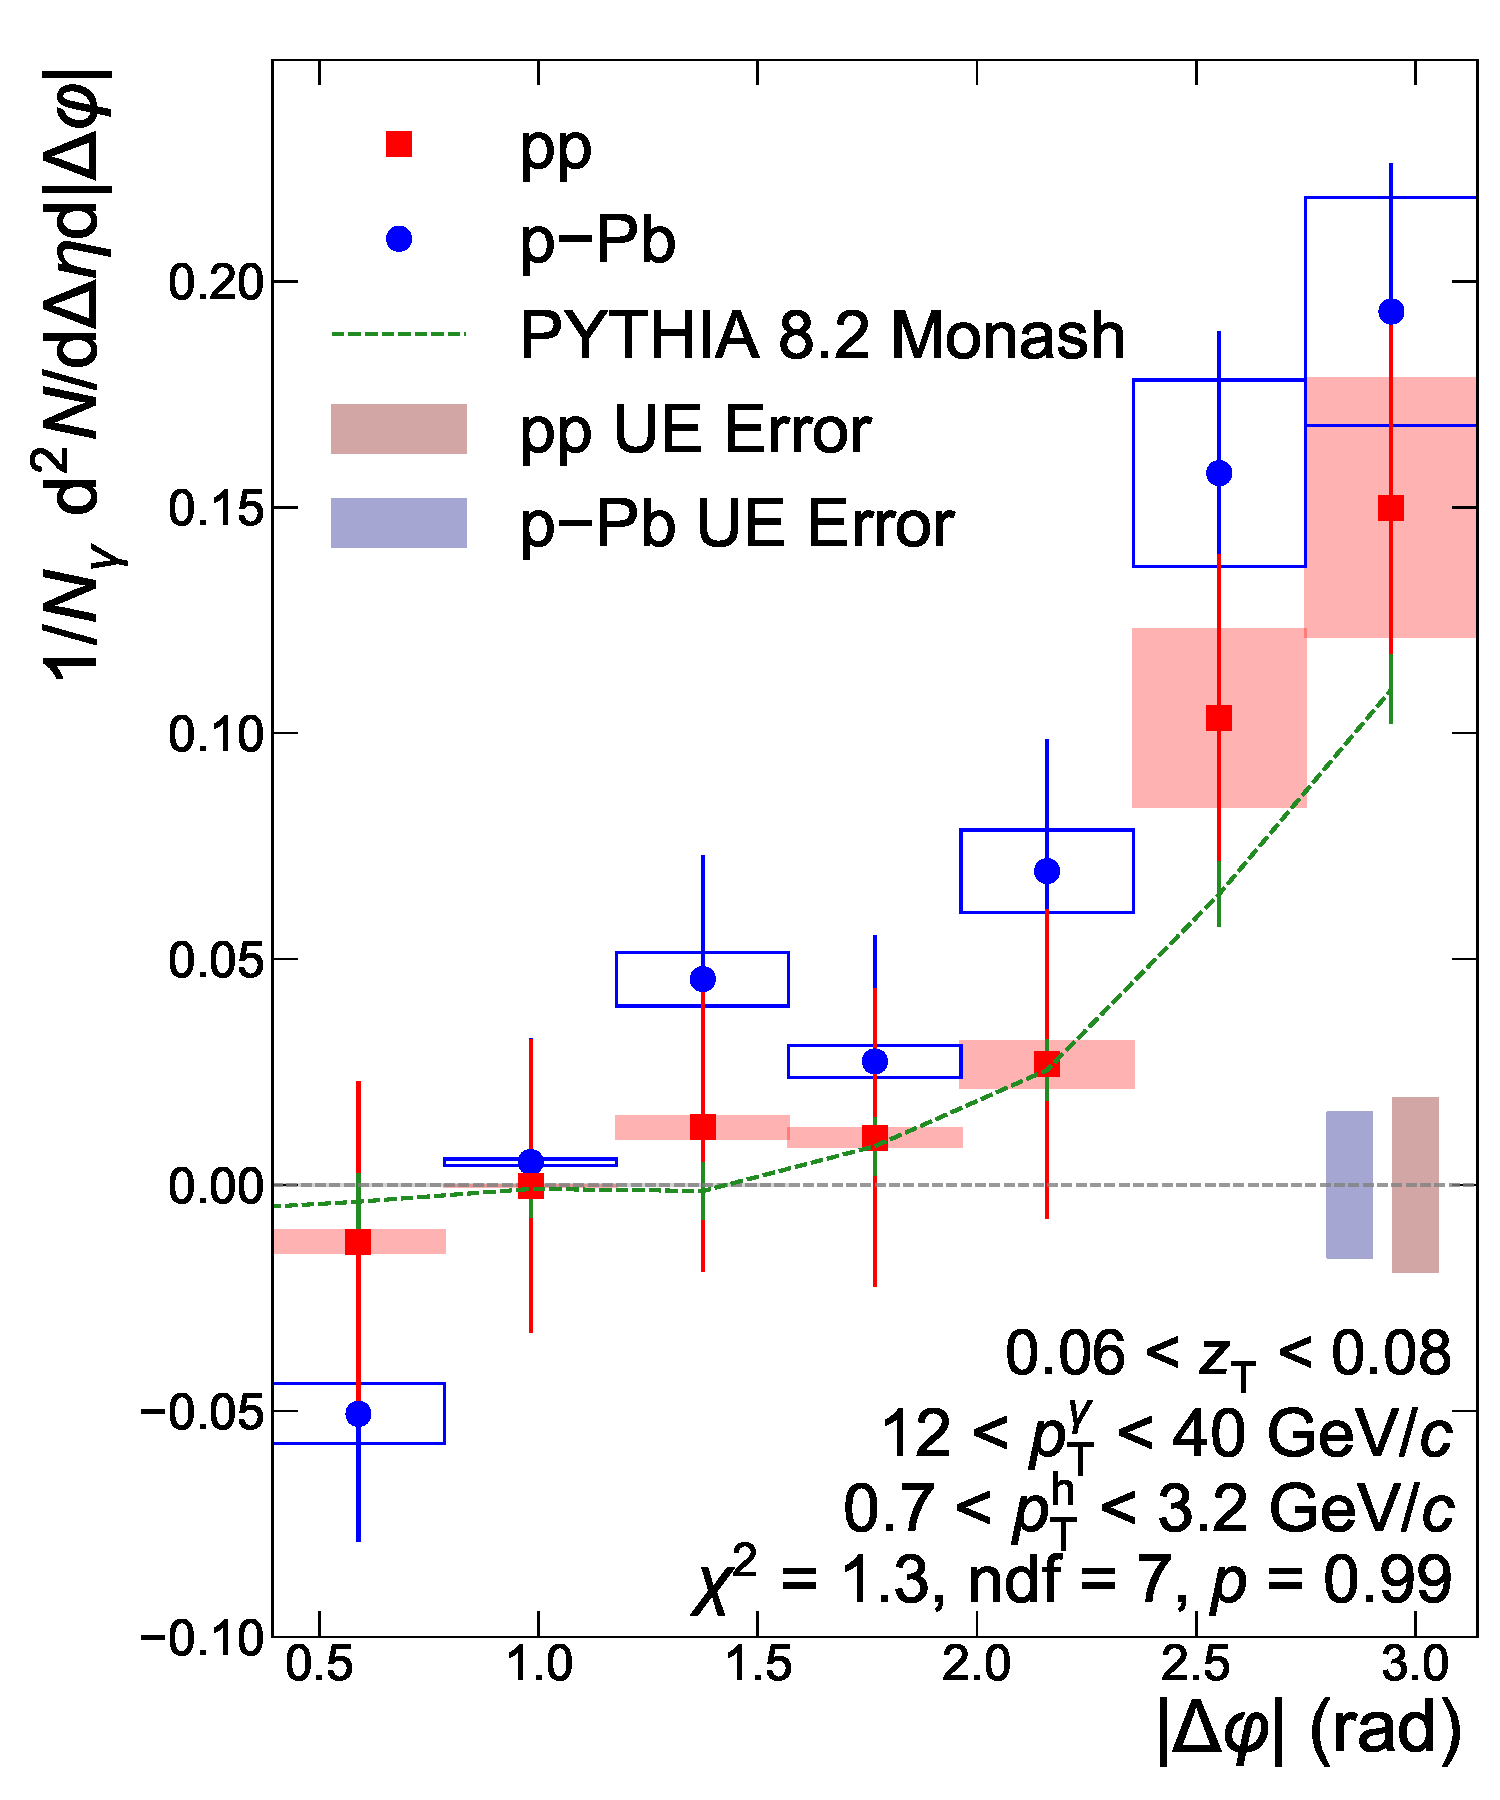
\includegraphics[width=0.3\textwidth]{Data_Analysis/gammahadron/Cs_Final_Indv_pT_0_zT_0.pdf}
    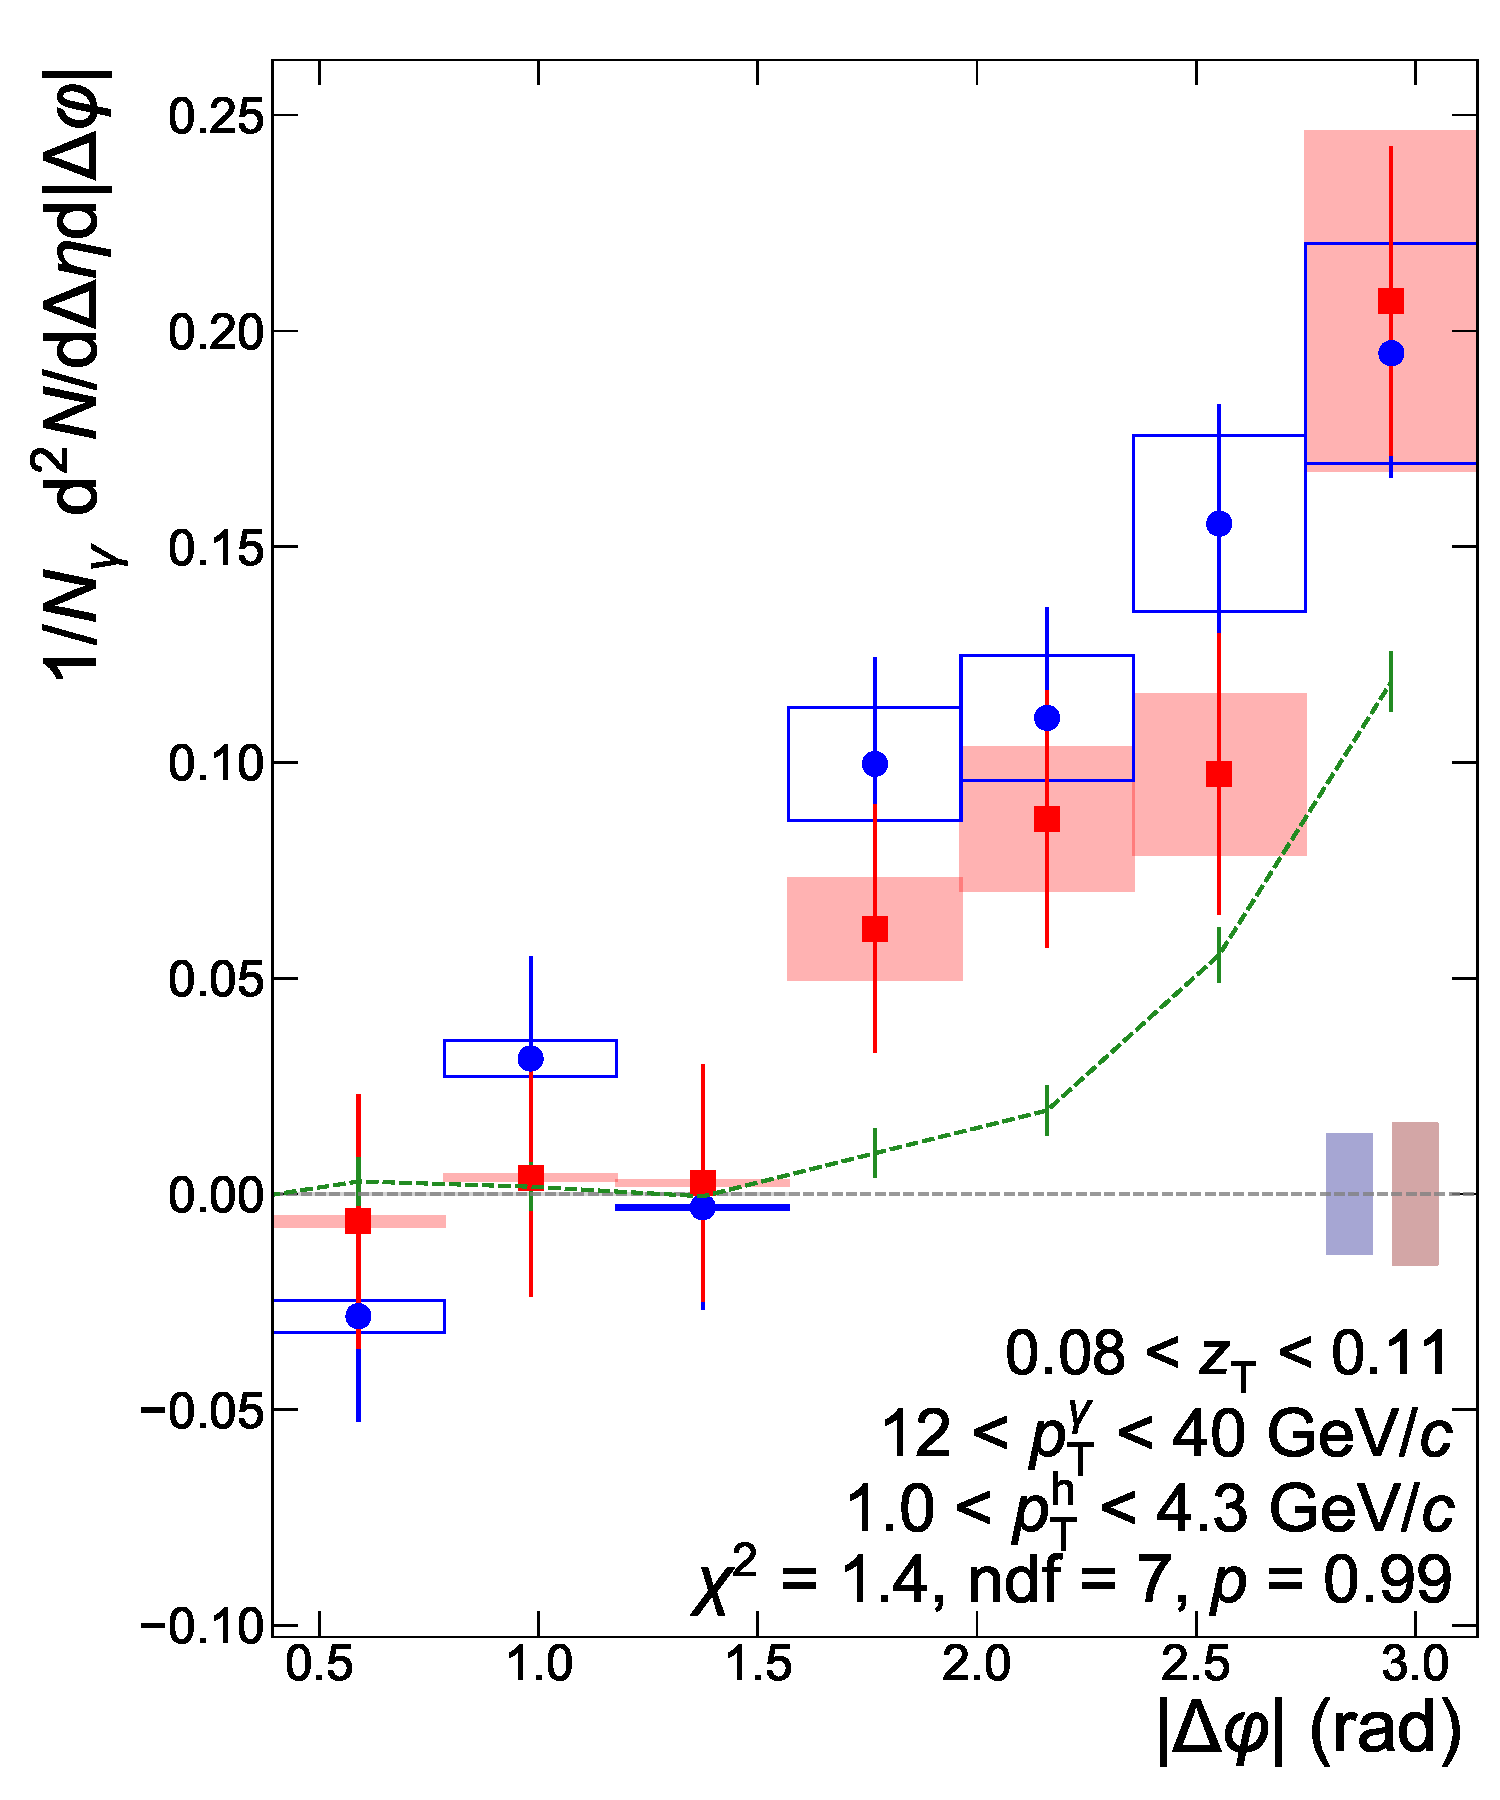
\includegraphics[width=0.3\textwidth]{Data_Analysis/gammahadron/Cs_Final_Indv_pT_0_zT_1.pdf}        
    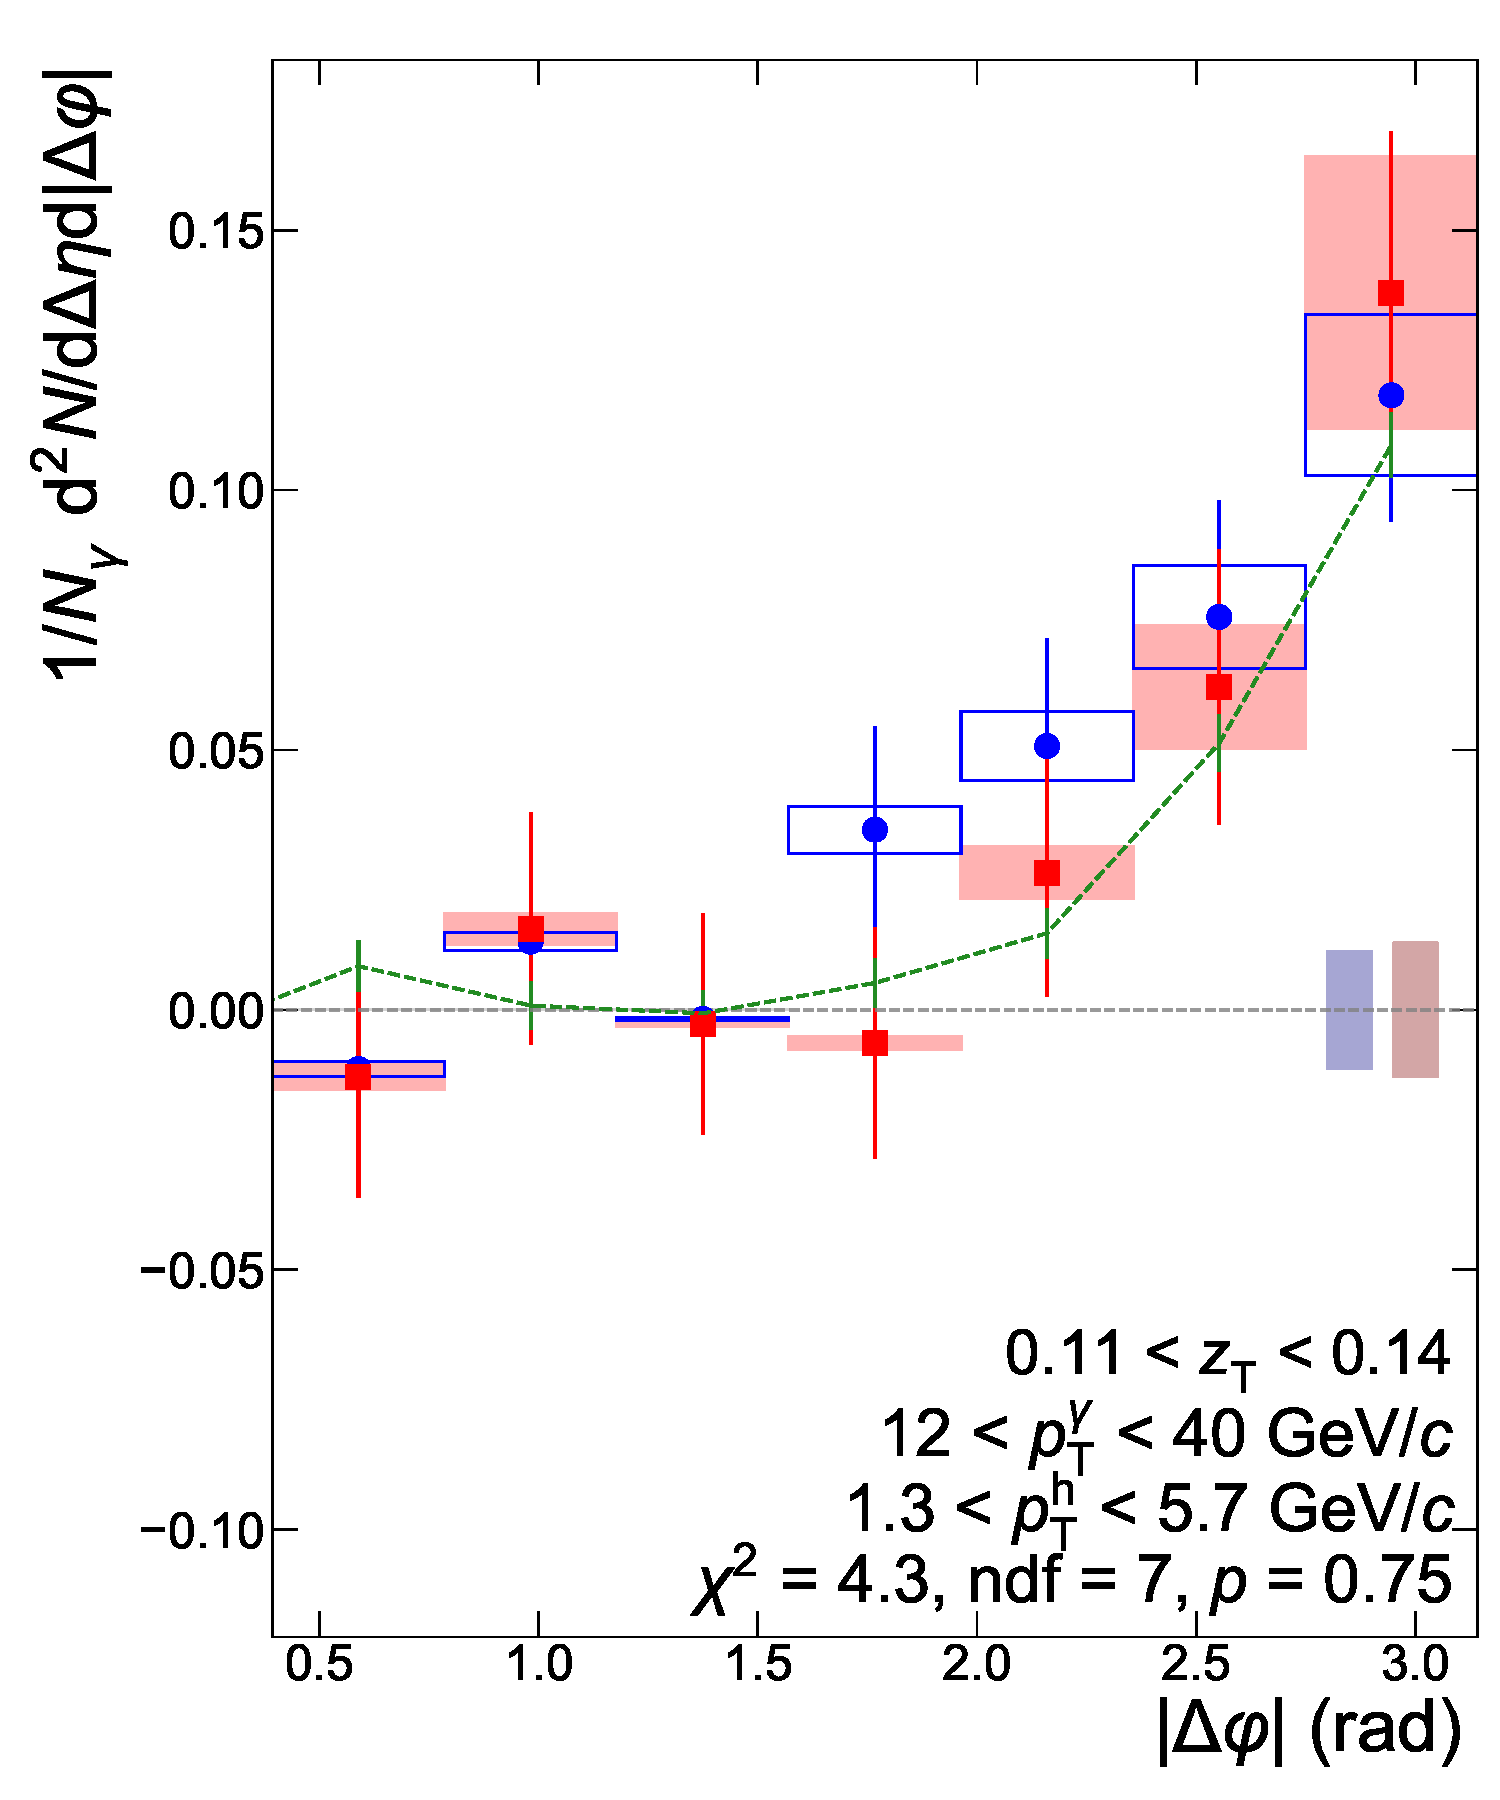
\includegraphics[width=0.3\textwidth]{Data_Analysis/gammahadron/Cs_Final_Indv_pT_0_zT_2.pdf}        
    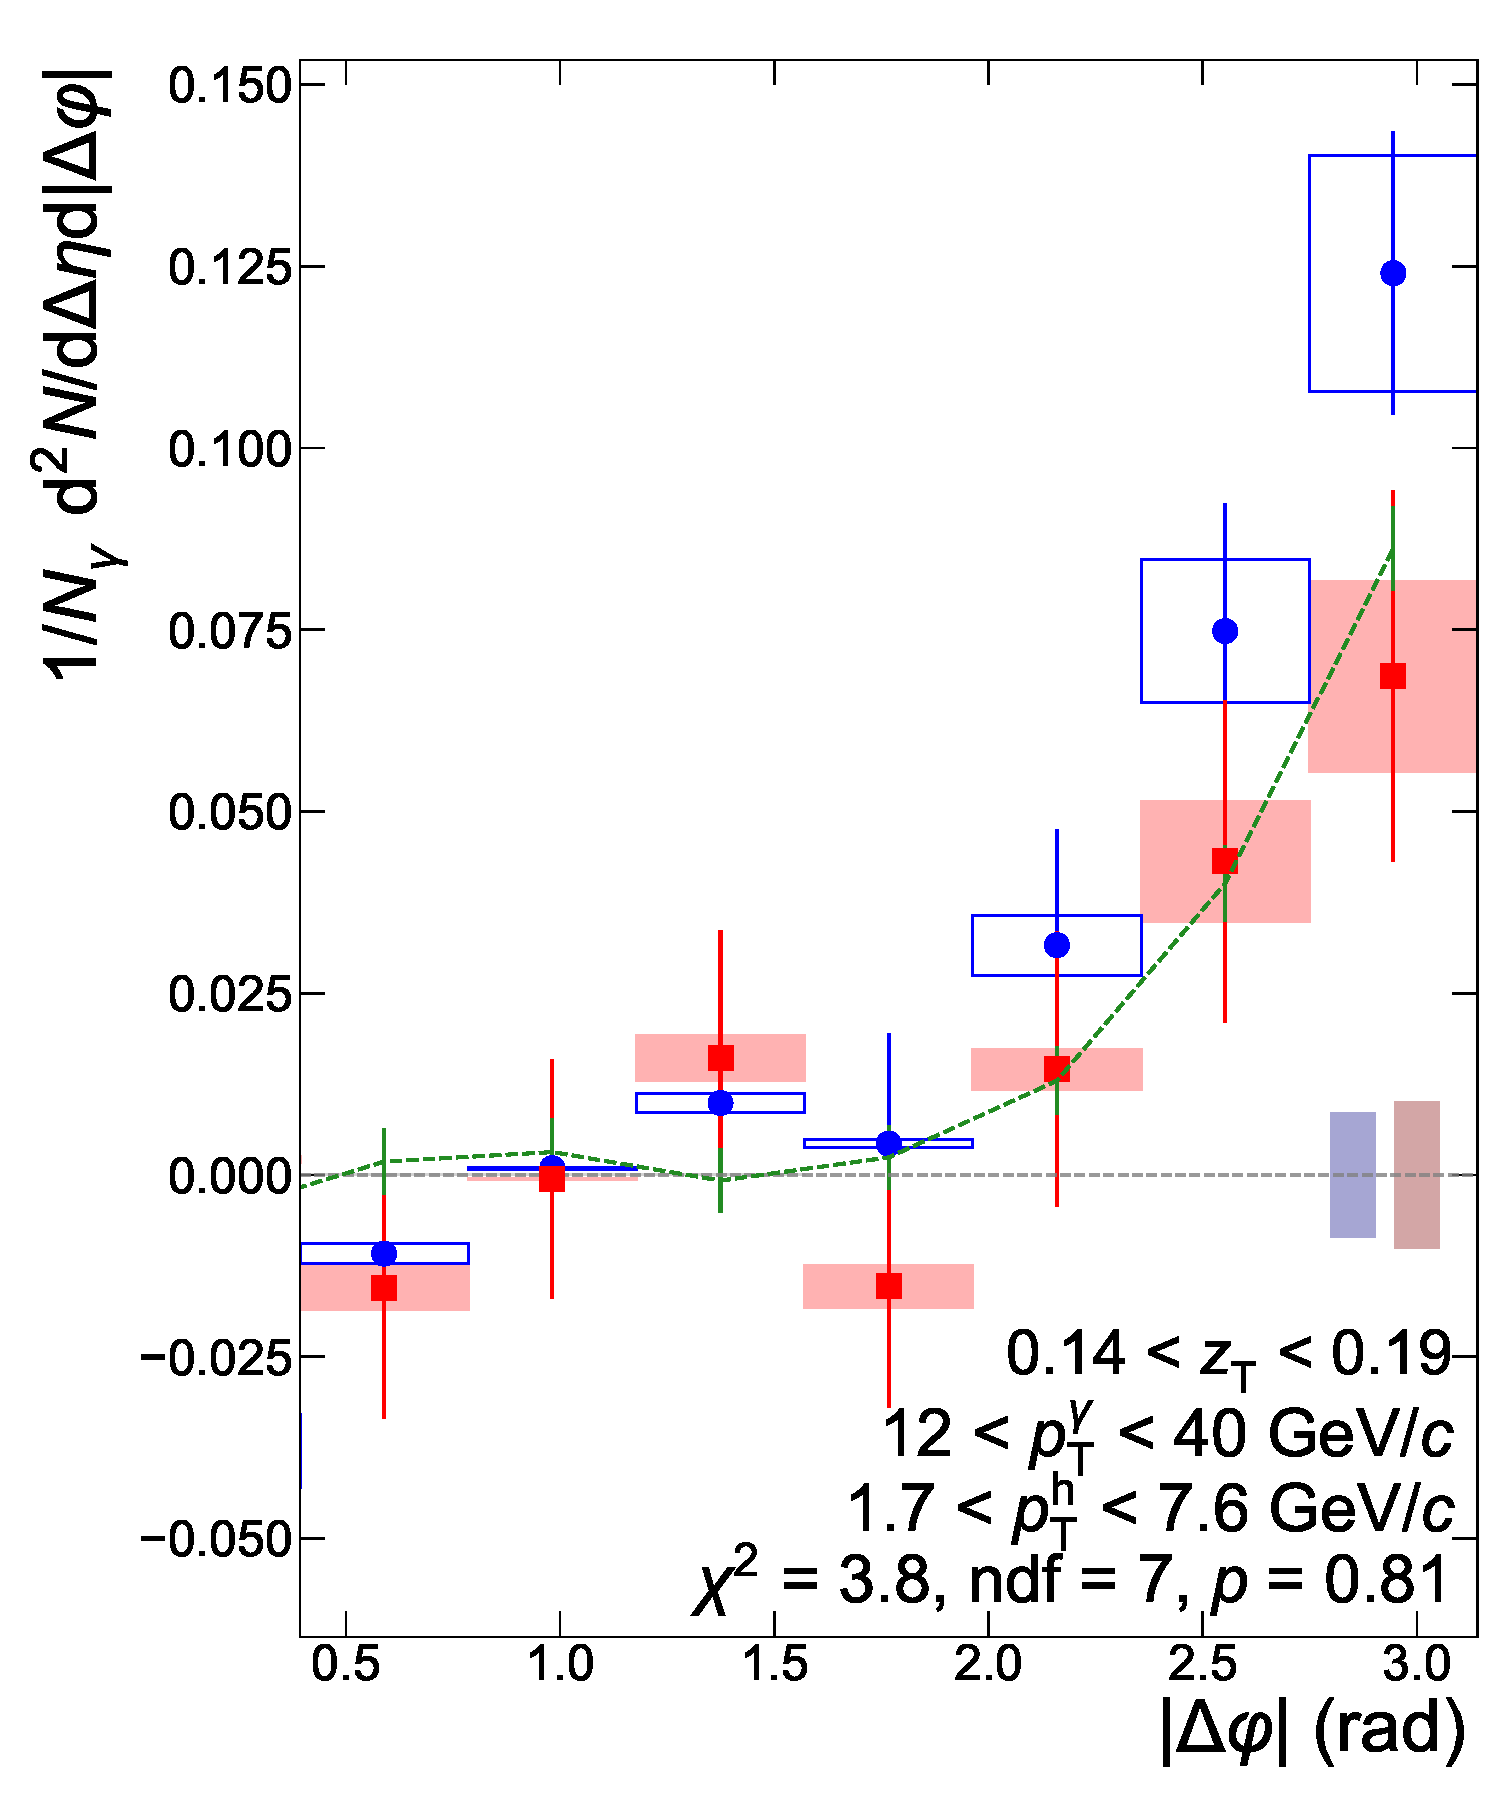
\includegraphics[width=0.3\textwidth]{Data_Analysis/gammahadron/Cs_Final_Indv_pT_0_zT_3.pdf}        
    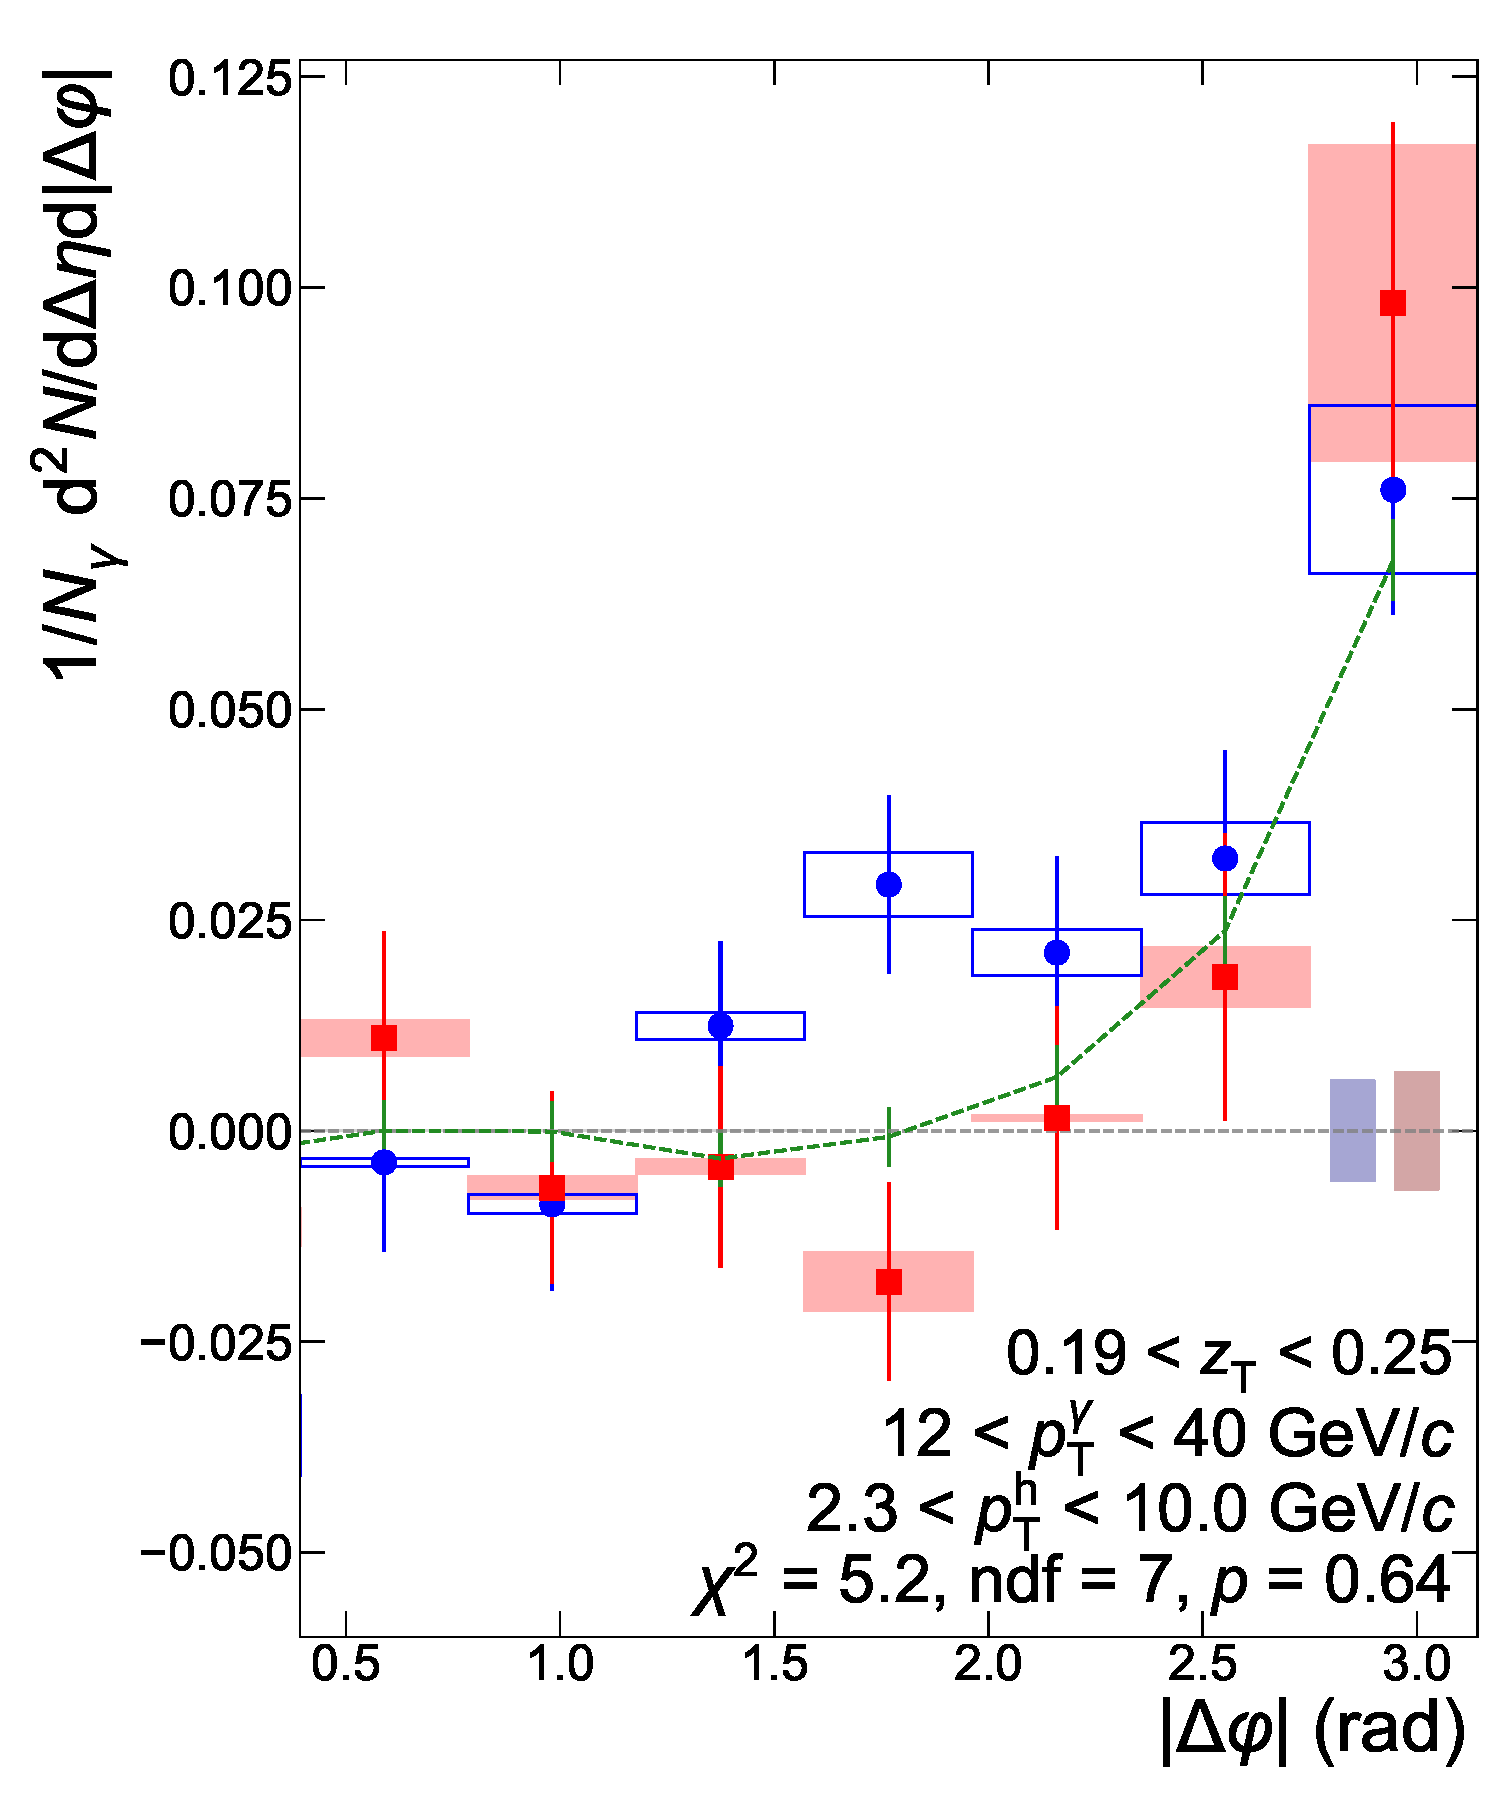
\includegraphics[width=0.3\textwidth]{Data_Analysis/gammahadron/Cs_Final_Indv_pT_0_zT_4.pdf}        
    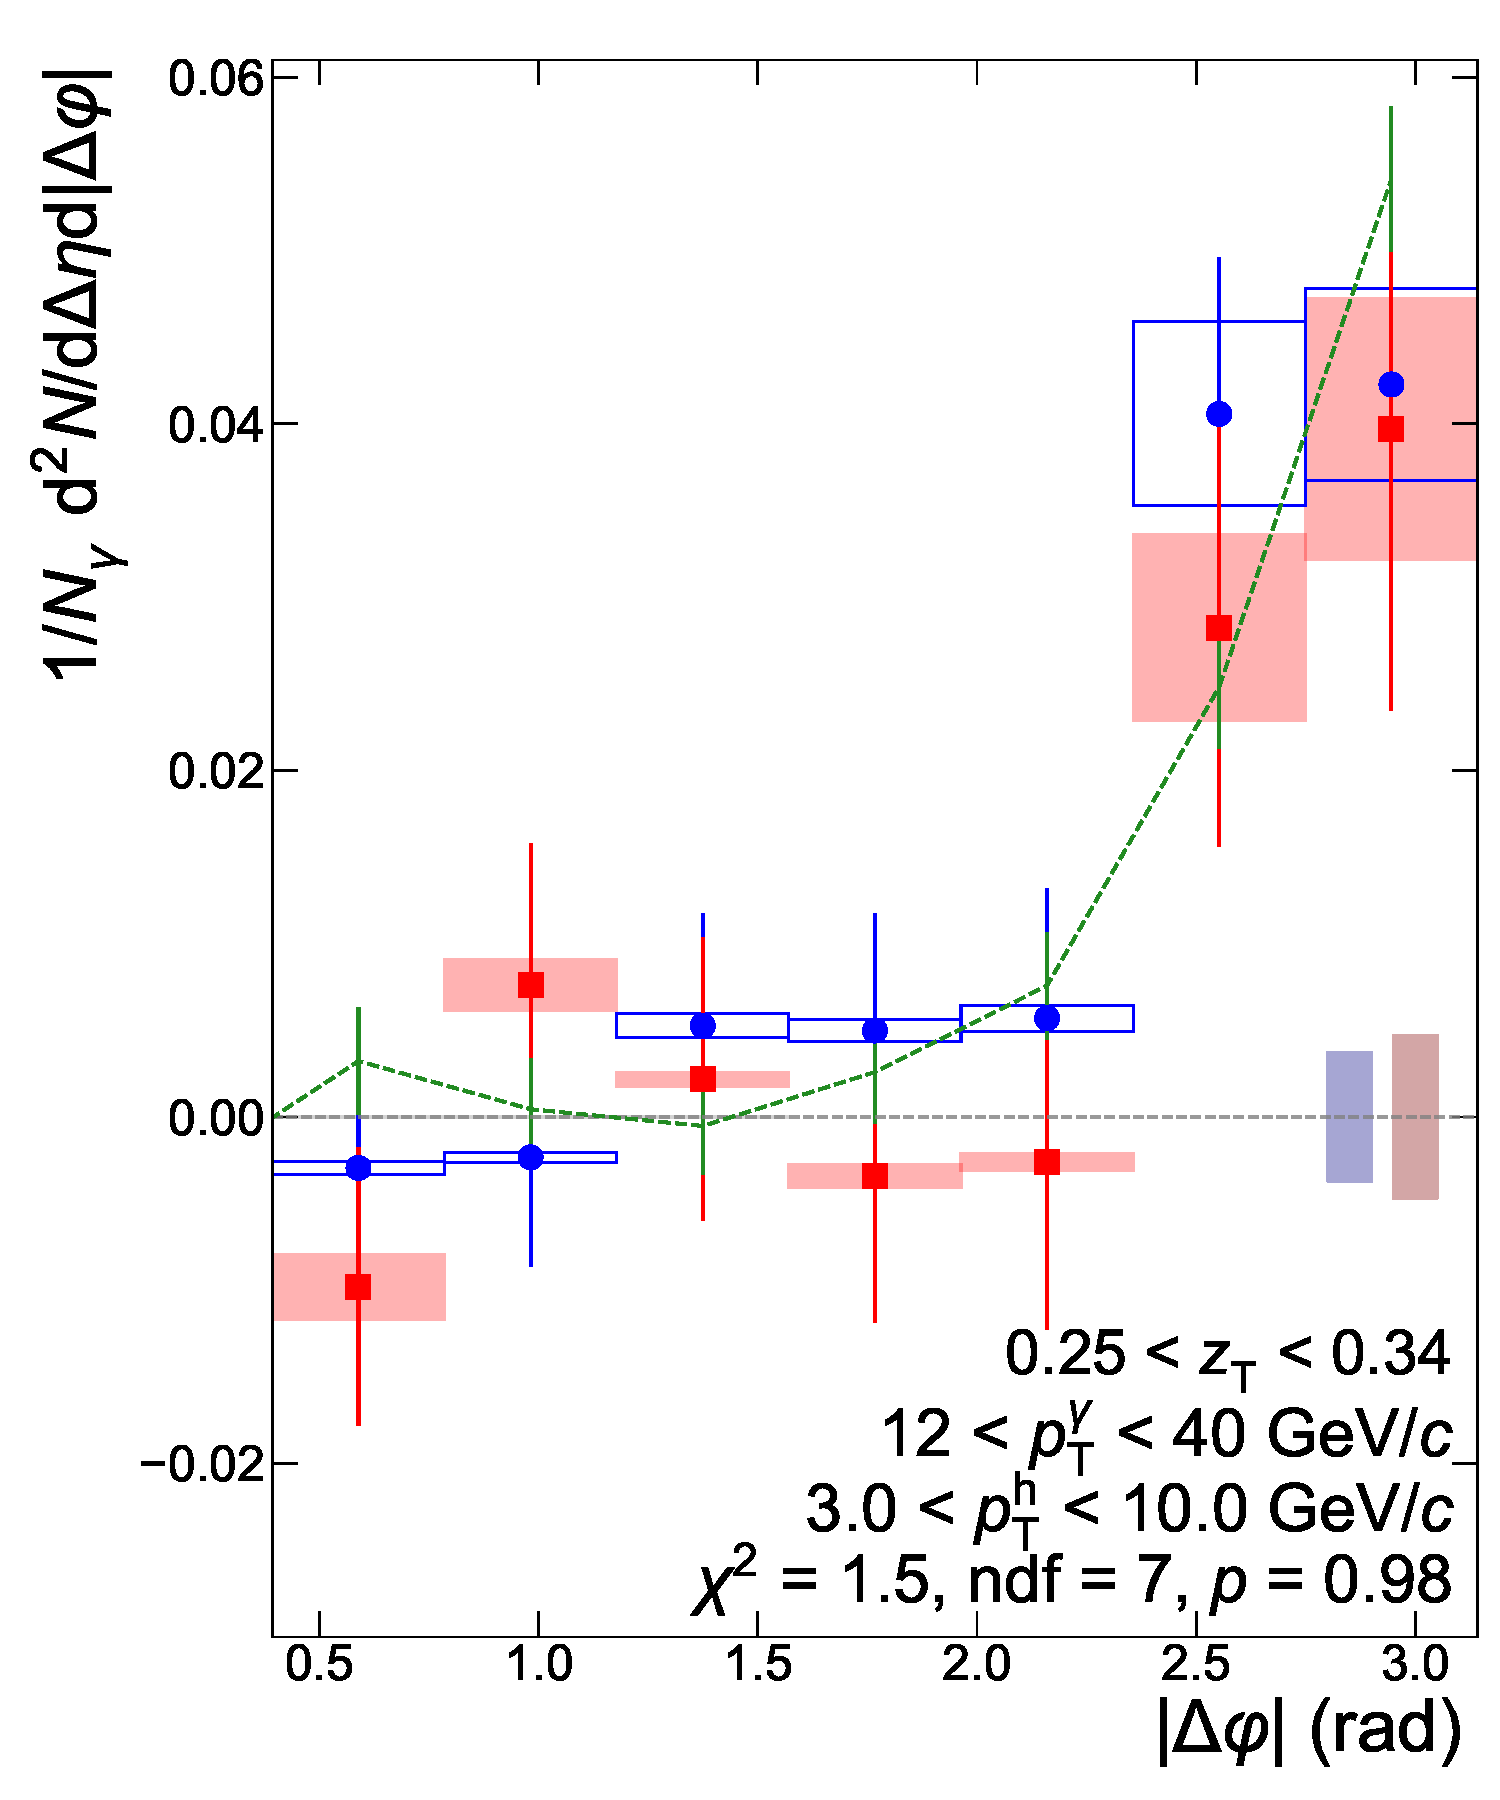
\includegraphics[width=0.3\textwidth]{Data_Analysis/gammahadron/Cs_Final_Indv_pT_0_zT_5.pdf}        
    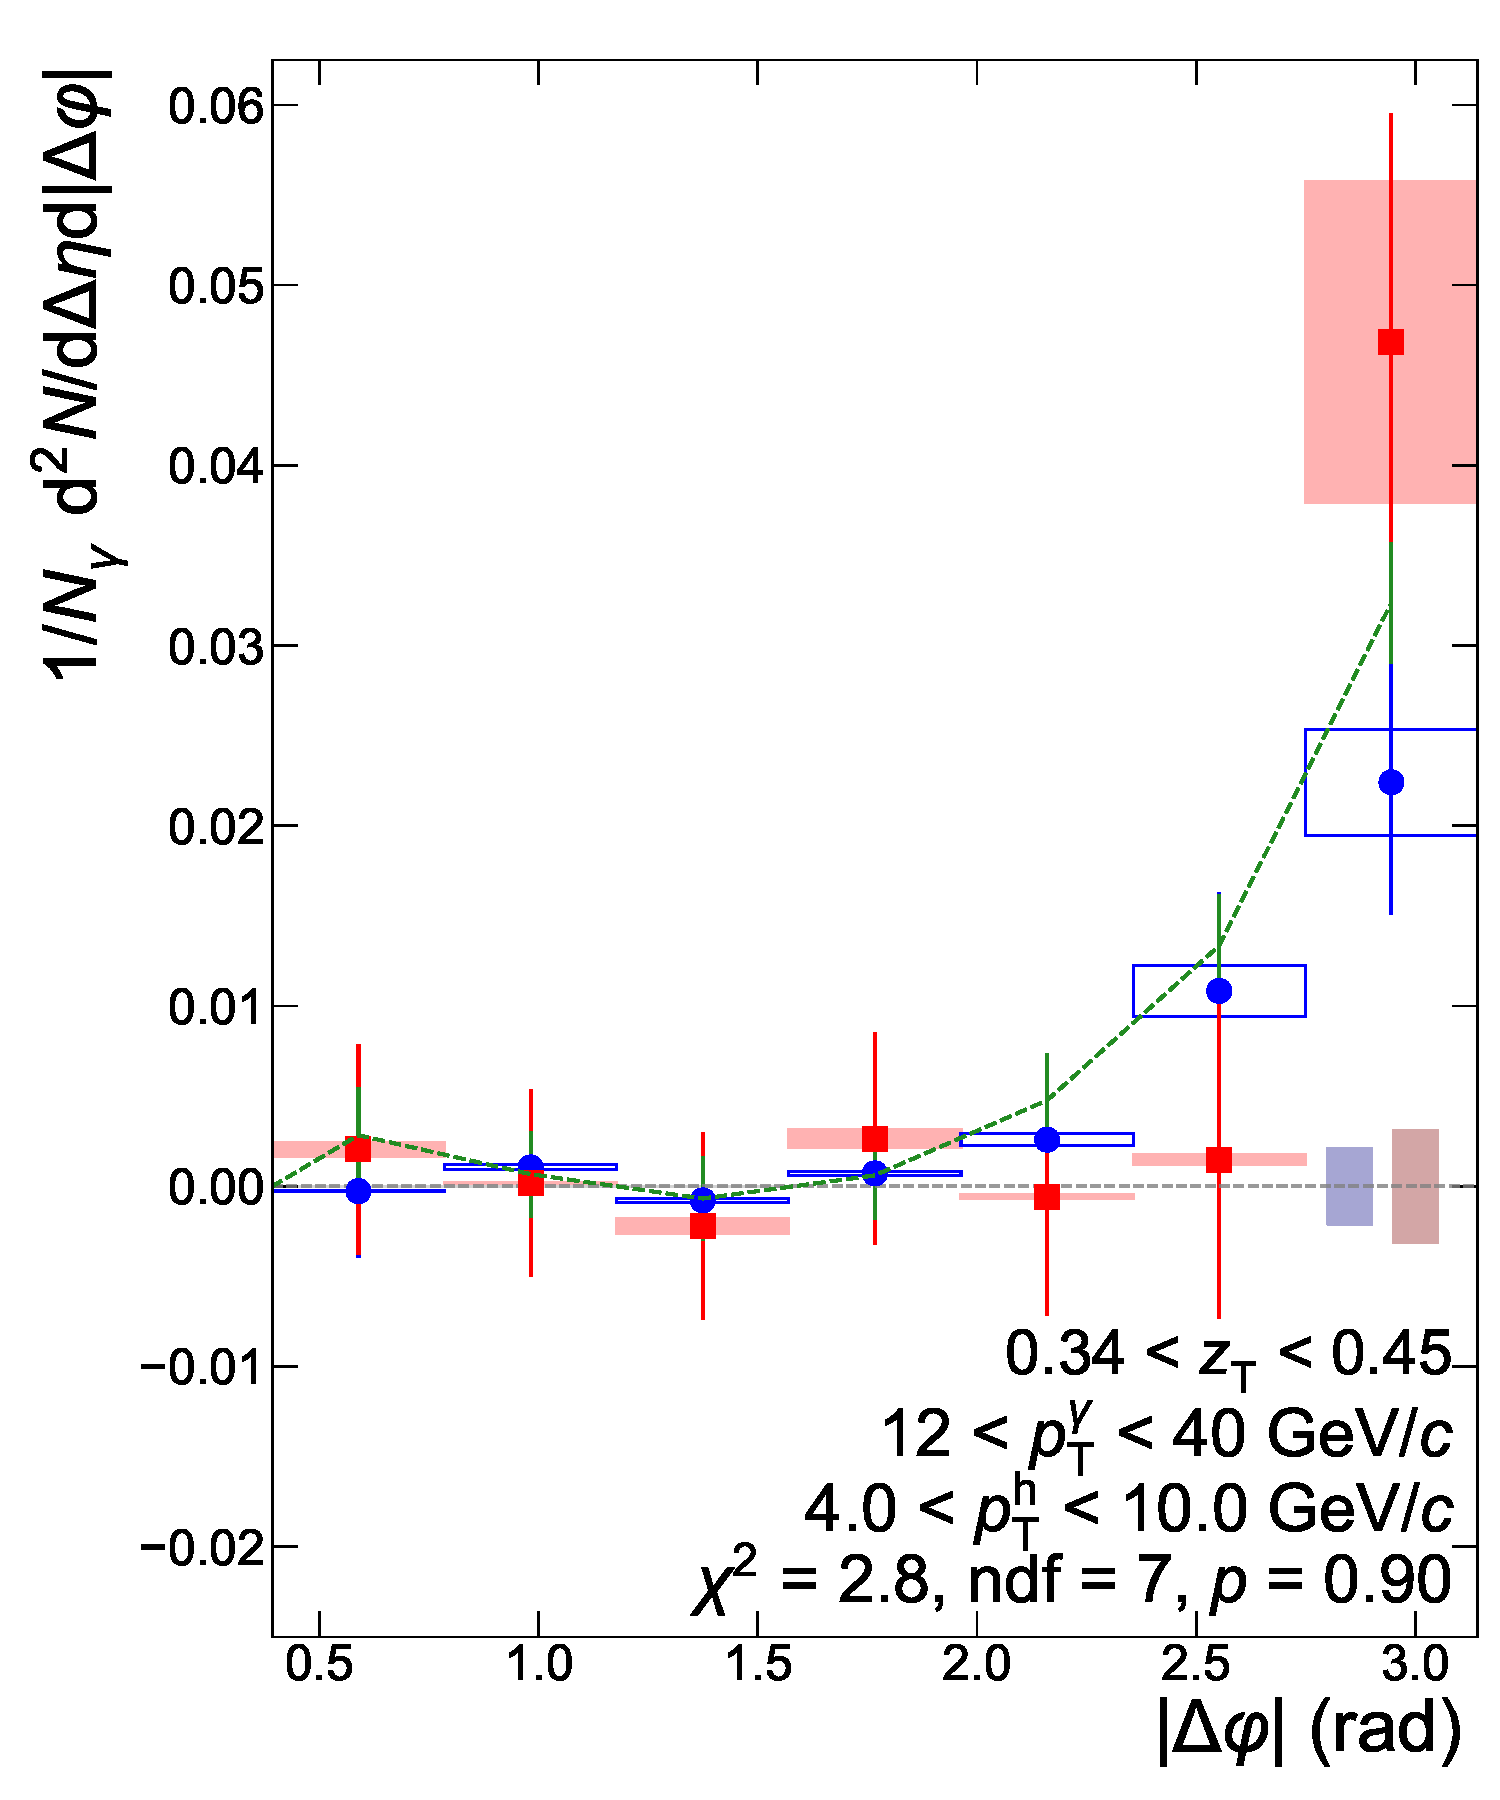
\includegraphics[width=0.3\textwidth]{Data_Analysis/gammahadron/Cs_Final_Indv_pT_0_zT_6.pdf}        
    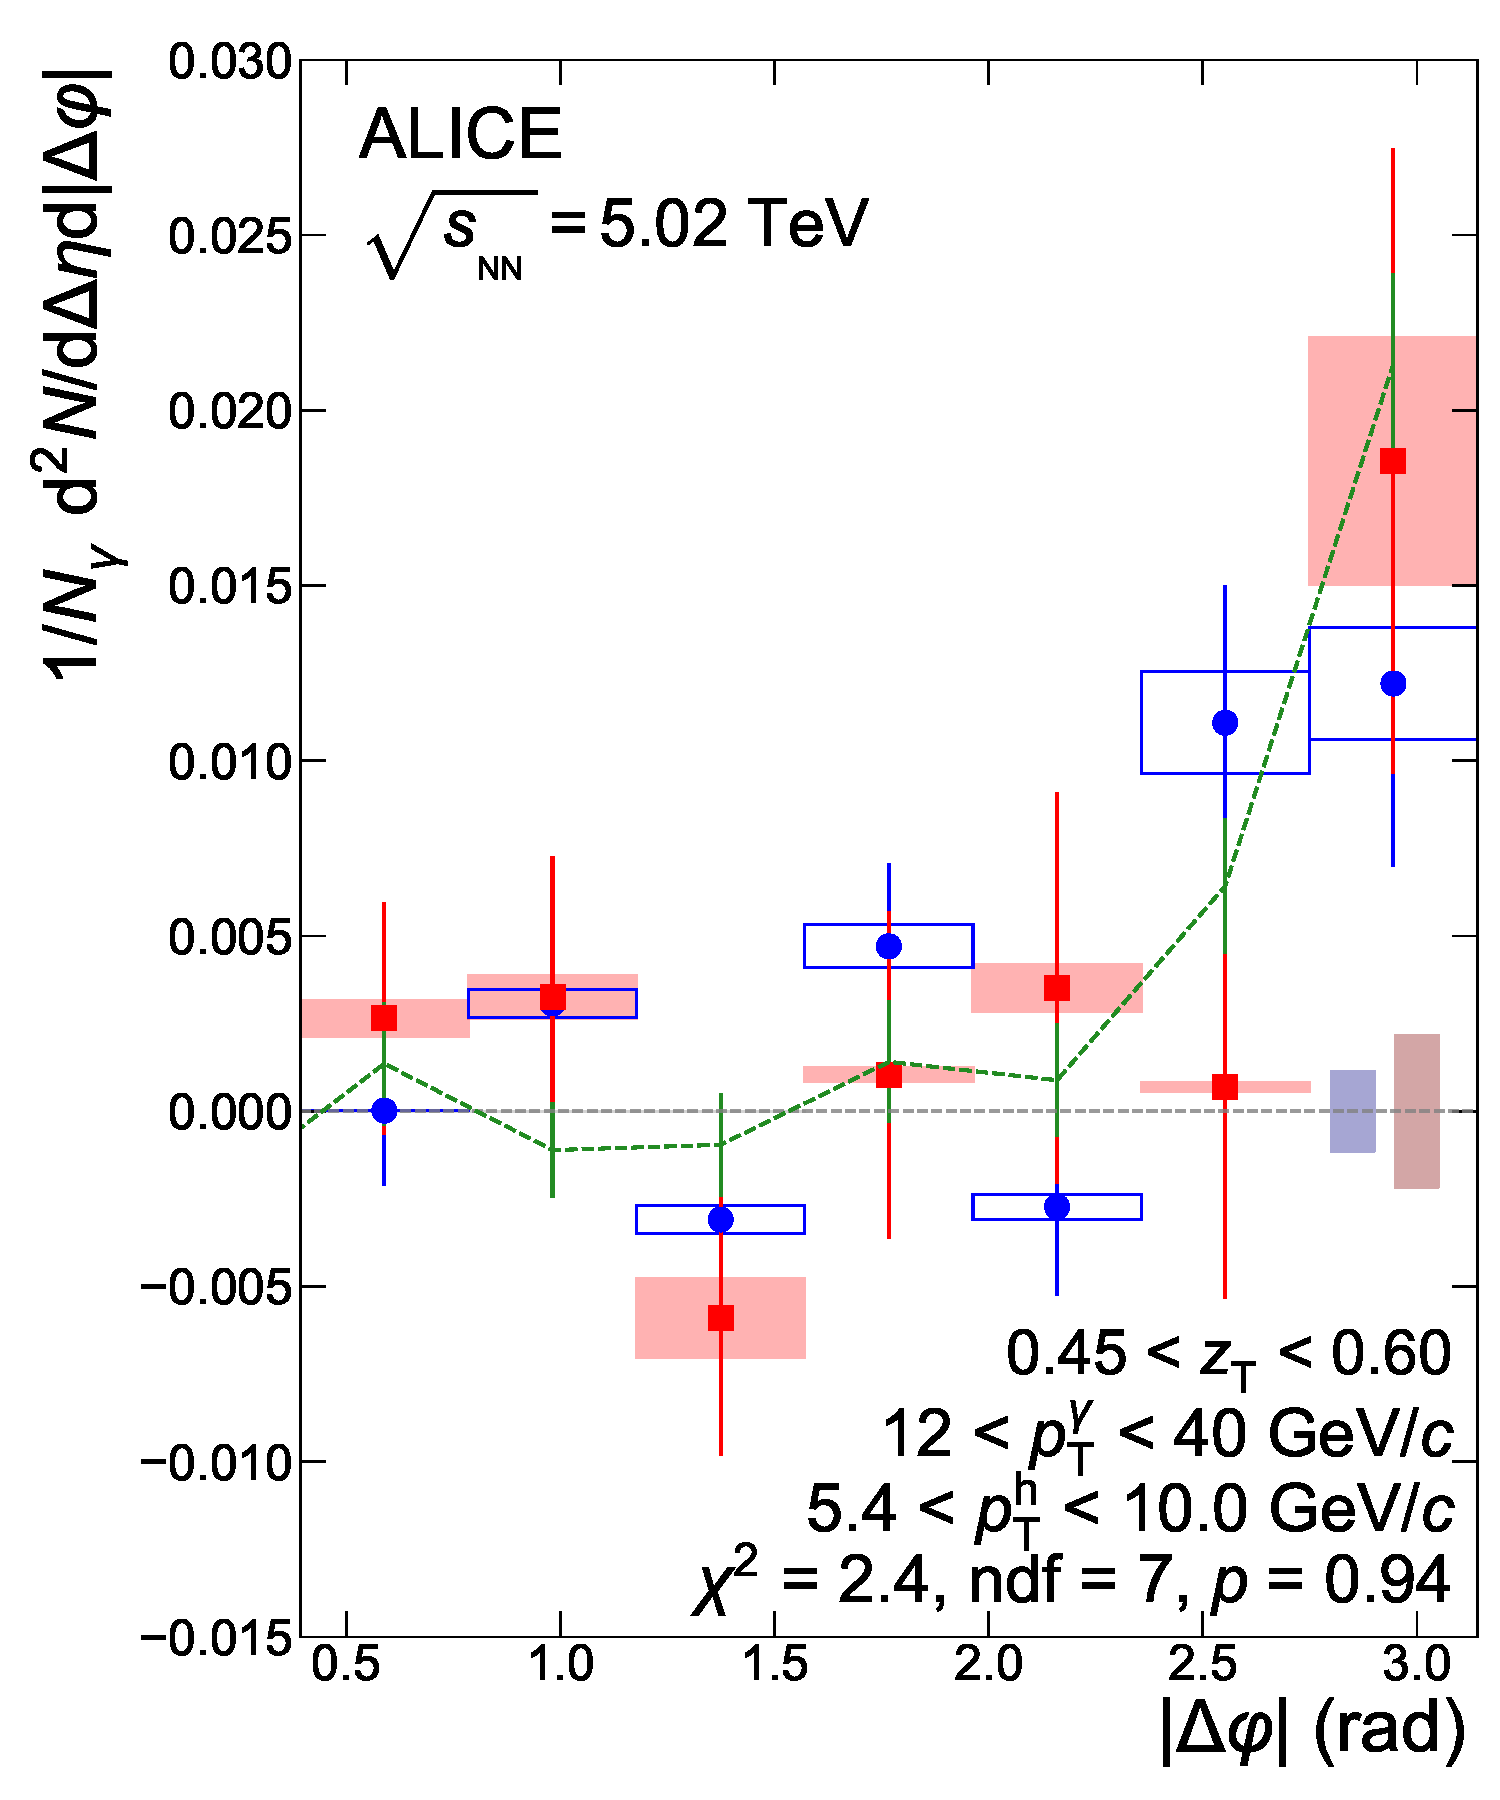
\includegraphics[width=0.3\textwidth]{Data_Analysis/gammahadron/Cs_Final_Indv_pT_0_zT_7.pdf}
    \caption{$\gammaiso$--hadron correlation functions for pp (red) and \pPb~(blue) data at $\sqrt{s_\mathrm{NN}}$ = 5.02 TeV as measured by the ALICE detector. The different panels represent three different \zt~bins. The correlation functions are projected over the range $|\Delta\eta| < 1.2$. The darker bands at zero represents the uncertainty from the underlying event estimation in pp and \pPb. The underlying event was estimated over the range $0.4 <|\Delta\varphi| < 1.6$. The vertical bars represent statistical uncertainties only. The boxes indicate the systematic uncertainties. The dashed green line represents the \gammaiso--hadron correlation function obtained with \textsc{PYTHIA 8.2} Monash Tune. ``$p$" is the p-value for the hypothesis that the pp and \pPb~data follow the same true correlation function.
    }
     \label{fig:GH_Correlations}
 \end{figure*}
\FloatBarrier

%\begin{figure*}
    %\centering
    %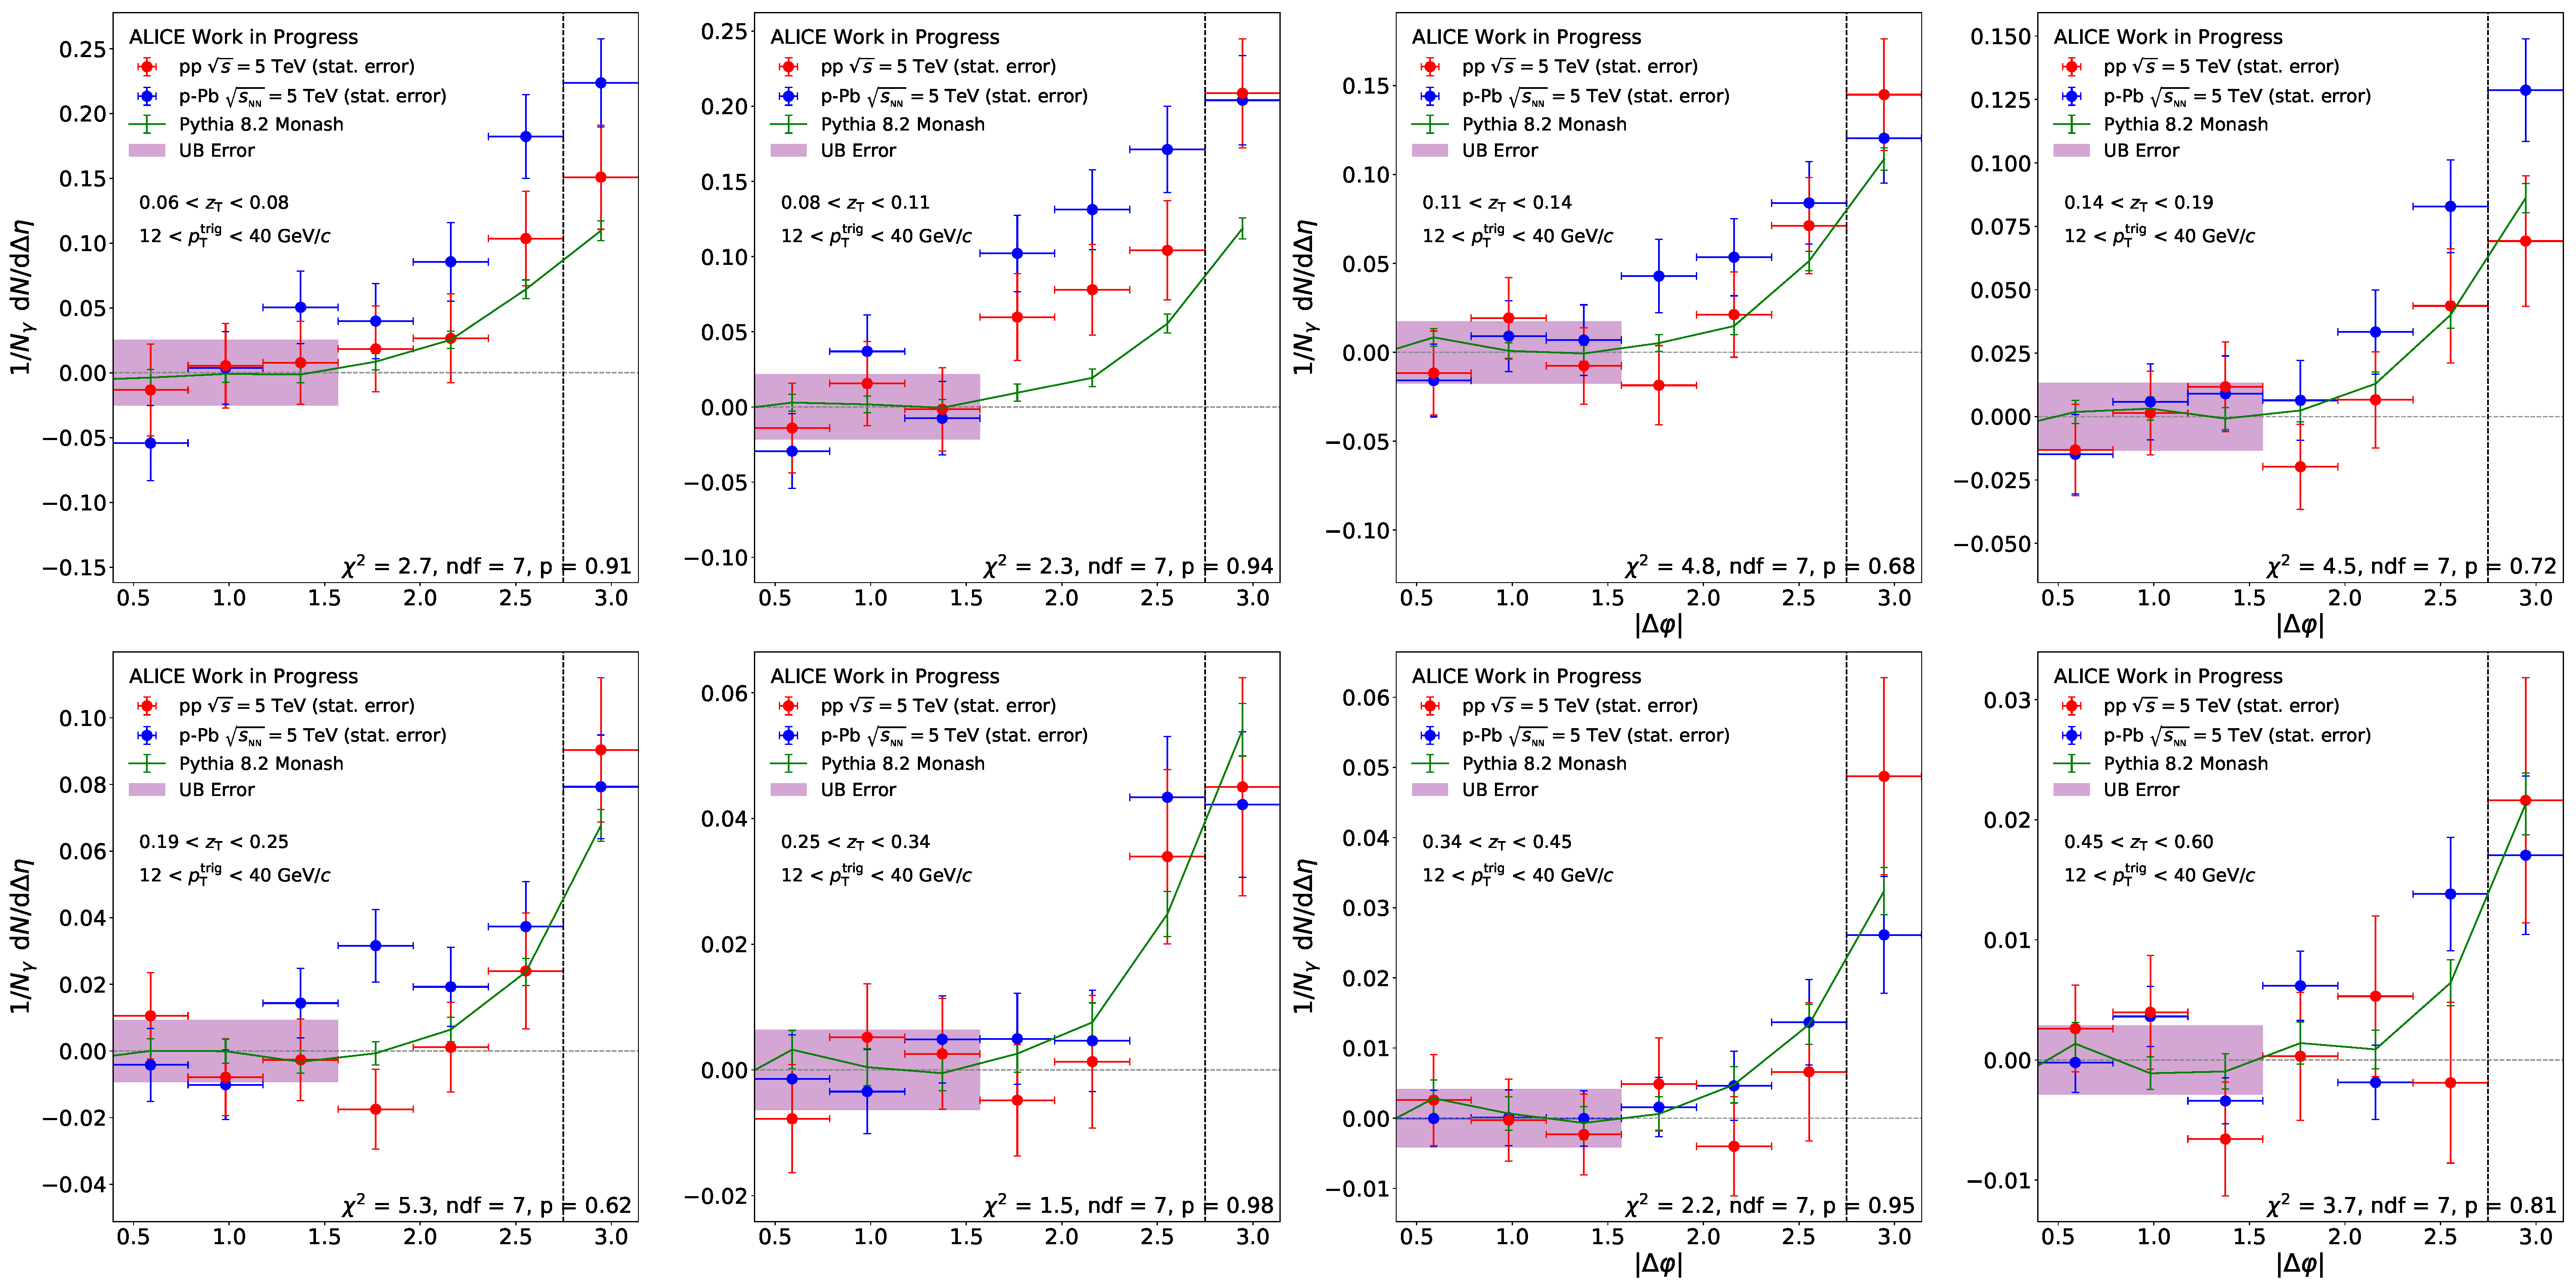
\includegraphics[width=1.0\textwidth]{gammahadron/Cs_Final_All_pT_0.pdf}        
    %\caption{$\gammaiso$--hadron correlation functions for pp (red) and \pPb~(blue) data at $\sqrt{s_\mathrm{NN}}$ = 5.02 TeV as measured by the ALICE detector. The different panels represent different \zt~bins. The purple band represents the uncertainty from the underlying event estimate n pp and \pPb. The vertical bars represent statistical uncertainty only. The horizontal bars represent the bin width in $\Delta\varphi$. The histogram is the \gammaiso--hadron correlation function obtained with \textsc{PYTHIA 8.2} Monash Tune. "p" is the p-value for the hypothesis that the pp and p-Pb data follow the same true correlation function}
%\end{figure*}

The darker colored bands at zero represents the uncertainty from the uncorrelated background estimate. The vertical bars indicate the statistical uncertainty only. The final correlation functions in each collision system demonstrate similar behavior: both show a signal consistent with zero at small $\Delta\varphi$, and a rising away-side peak at large $\Delta\varphi$ arising predominantly from the hard-scattered parton opposite to the trigger photon.
%$\gammaiso$.

Agreement within uncertainties between pp, \pPb, and the \textsc{PYTHIA 8.2} Monash Tune is observed.
By measuring associated hadrons, correlations can be observed at much larger angles than would otherwise be possible for hadrons within a reconstructed jet. A $\chi^2$ test between pp and \pPb~data and a p-value is calculated in each \zt~bin for the null hypothesis that pp and \pPb~data follow the same true correlation function. In each bin, the null hypothesis cannot be rejected, indicating that there is no significant difference between the correlation functions in the two collision systems.

\section{Parton Fragmentation Function}
As discussed in Sec.~\ref{sec:intro_gh}, the correlation functions from Fig. \ref{fig:GH_Correlations} are then integrated in the region $|\Delta\varphi| > \frac{7\pi}{8}$ for each $\zt$~bin in order to obtain the $\gammaiso$-tagged fragmentation function shown in Fig. \ref{fig:Fragmentation_Functions}. This range roughly corresponds to the azimuthal angle consistent with the commonly used radius of $R=$ 0.4 for jet measurements.

\begin{figure}
    \centering
    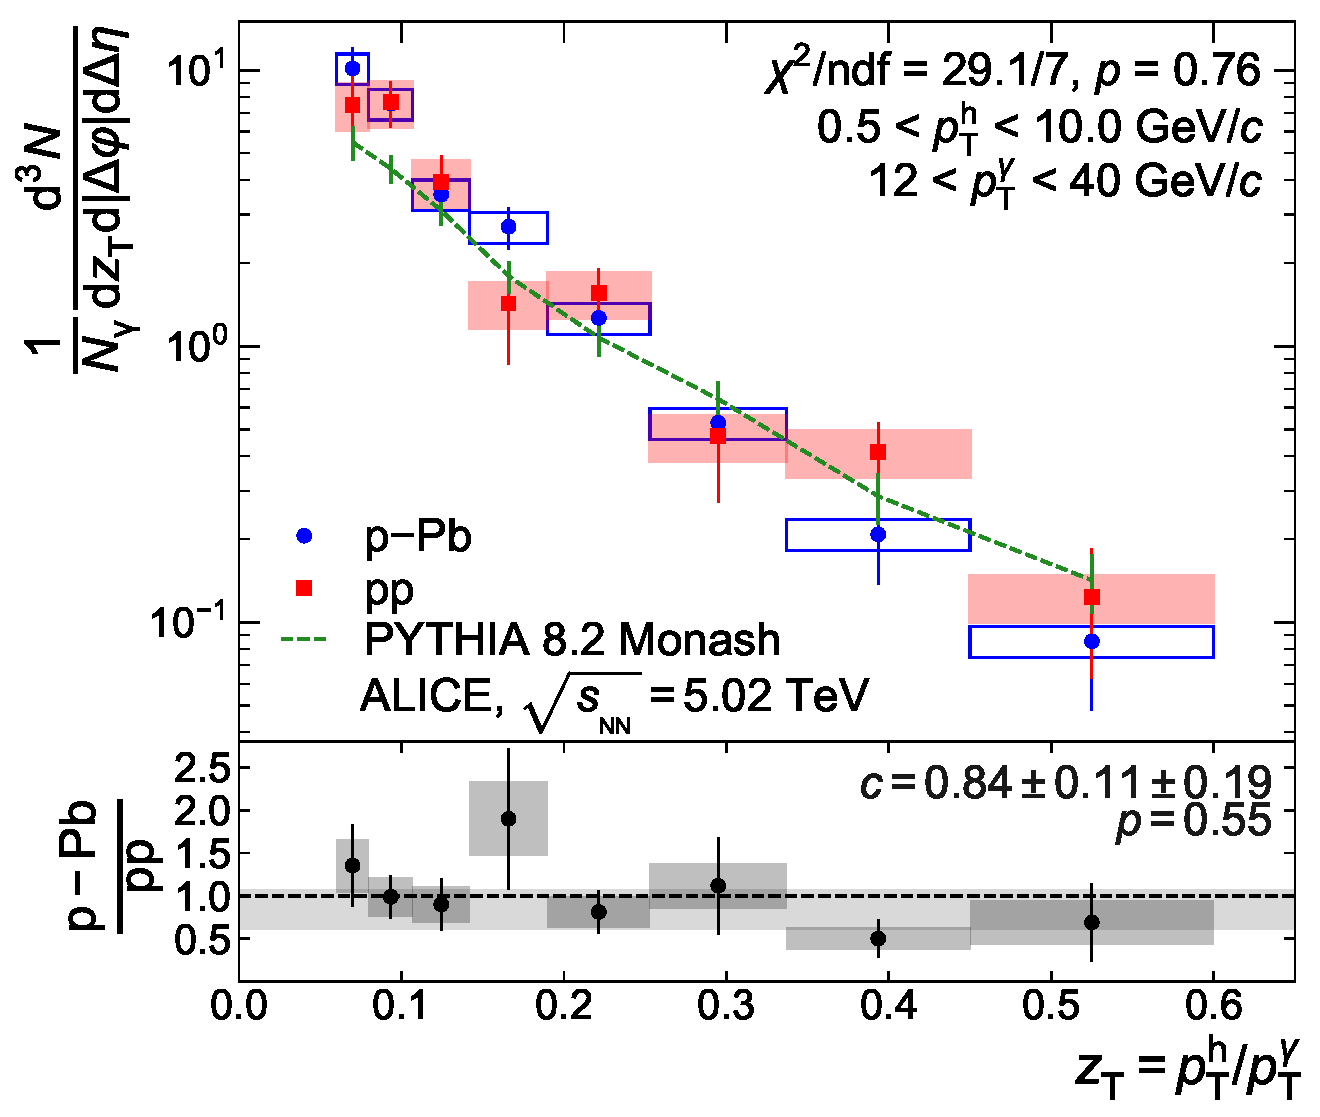
\includegraphics[width=0.67\textwidth]{Data_Analysis/gammahadron/Final_FFunction_and_Ratio.pdf}
    \caption{$\gammaiso$-tagged fragmentation function for pp (red) and \pPb~data (blue) at $\sqrt{s_\mathrm{NN}}$ = 5.02 TeV as measured by the ALICE detector. The boxes represent the systematic uncertainties while the vertical bars indicate the statistical uncertainties. The dashed green line corresponds to \textsc{PYTHIA 8.2}. The $\chi^2$ test for the comparison of pp and \pPb~data incorporates correlations among different \zt~intervals. A constant that was fit to the ratio including statistical and systematic uncertainties is shown as grey band, with the width indicating the uncertainty on the fit.}
    \label{fig:Fragmentation_Functions}
\end{figure}

The statistical uncertainty on the away-side yields in each $\zt$~bin is calculated from the statistical uncertainty in the fully subtracted correlation functions, along with the statistical uncertainty arising from the uncorrelated background subtraction. A maximum charged hadron \pt~of 10 \GeVc~and a photon trigger \pt~up to 40 \GeVc~could result in a potential bias of the associated \zt~spectrum. However, by repeating the analysis in different photon trigger \pt~bins, it was found that any such effects were negligible compared to other uncertainties. The two largest sources of systematic uncertainty are from the purity and the single track correction factors. For the chosen $\pt^{\mathrm{track}}$ interval, there is no strong $\pt$~dependence for the uncertainty of the charged tracking efficiency.

 The ratio of the fragmentation functions in \pPb~ and pp collisions is shown in the lower panel of Fig.~\ref{fig:Fragmentation_Functions}.
The fit yields a constant factor of $0.84\pm0.11\mathrm{(stat)}\pm0.19\mathrm{(sys)}$, with a reduced $\chi^{2}$ of 0.84.  
 Thus, within total uncertainties, ranging from 22--40\% for different \zt~bins the \pPb~to pp ratio is consistent with unity. %Thus, within approximately 23--40\% these uncertainties, the fragmentation function in \pPb collisions is the same as in pp collisions.

% \begin{table}
%    \centering
%    \caption{Summary of uncertainties on integrated away side yields in proton-lead and proton-proton collisions. The uncertainties quoted are absolute.} 
%    \begin{tabular*}{1.0\columnwidth}{@{\extracolsep{\fill}}llc@{}}
%     \hline
% $z_\mathrm{T}$ Range & pp $\pm$ Stat. $\pm$ Sys & p--Pb $\pm$ Stat. $\pm$ Sys. \\
% \hline
% 0.06--0.08 & 7.50$ \pm$ 2.23 $\pm$1.42 & 9.67$ \pm$ 1.82 $\pm$1.27 \\
% 0.08--0.11 & 7.66$ \pm$ 1.46 $\pm$1.46 & 7.22$ \pm$ 1.18 $\pm$0.94 \\
% 0.11--0.14 & 3.94$ \pm$ 0.96 $\pm$0.75 & 3.38$ \pm$ 0.76 $\pm$0.44 \\
% 0.14--0.19 & 1.43$ \pm$ 0.57 $\pm$0.27 & 2.58$ \pm$ 0.44 $\pm$0.34 \\
% 0.19--0.25 & 1.56$ \pm$ 0.36 $\pm$0.30 & 1.21$ \pm$ 0.25 $\pm$0.16 \\
% 0.25--0.34 & 0.47$ \pm$ 0.20 $\pm$0.09 & 0.50$ \pm$ 0.14 $\pm$0.07 \\
% 0.34--0.45 & 0.41$ \pm$ 0.12 $\pm$0.08 & 0.20$ \pm$ 0.07 $\pm$0.03 \\
% 0.45--0.60 & 0.12$ \pm$ 0.06 $\pm$0.02 & 0.08$ \pm$ 0.04 $\pm$0.01 \\
%   \end{tabular*}
%    \label{tab:FF_Summary}
% \end{table}


% \begin{table}[h]
%    \centering
%    \caption{Number of $\gammaiso$--hadron pairs per $\gammaiso$ integrated in $\Delta\varphi>7\pi/8$, for different $\zt$ intervals. The uncertainty quoted is statistical only. } 
%    \begin{tabular*}{1.0\columnwidth}{@{\extracolsep{\fill}}lccc@{}}
%     \hline
% $\zt$ range & pp & \pPb & \pPb/pp \\
% \hline
% 0.06 - 0.08 & 7.496 $\pm$ 2.230 & 9.666 $\pm$ 1.818 & 1.290 $\pm$ 0.454 \\
% 0.08 - 0.11 & 7.663 $\pm$ 1.457 & 7.216 $\pm$ 1.182 & 0.942 $\pm$ 0.236 \\
% 0.11 - 0.14 & 3.943 $\pm$ 0.959 & 3.379 $\pm$ 0.765 & 0.857 $\pm$ 0.285 \\
% 0.14 - 0.19 & 1.429 $\pm$ 0.571 & 2.584 $\pm$ 0.443 & 1.809 $\pm$ 0.786 \\
% 0.19 - 0.25 & 1.559 $\pm$ 0.356 & 1.207 $\pm$ 0.253 & 0.774 $\pm$ 0.240 \\
% 0.25 - 0.34 & 0.473 $\pm$ 0.201 & 0.503 $\pm$ 0.135 & 1.065 $\pm$ 0.536 \\
% 0.34 - 0.45 & 0.415 $\pm$ 0.116 & 0.198 $\pm$ 0.068 & 0.478 $\pm$ 0.211 \\
% 0.45 - 0.60 & 0.124 $\pm$ 0.061 & 0.081 $\pm$ 0.036 & 0.658 $\pm$ 0.434 \\
	
% \hline 
%    \end{tabular*}
%    \label{tab:ff}
% \end{table}

% Figure~\ref{ffRatio} shows the ratio of \pPb~to pp data. The systematic uncertainties in the ratio are described in Section~\ref{sec:systematics}. The uncertainty due to UE-subtraction is fully uncorrelated with $\zt$ and is combined in quadrature with the statistical uncertainty and shown as bars. All other uncertainties are correlated with $\zt$ and shown in boxes. 


% \subsection{\pPb to pp ratio}
% \subsection{Integration Window}
% \subsection{Cold nuclear matter measurements at future EIC}
% \subsection{Transverse Momentum Dependent Distributions}
% \subsection{Probing $\hat{q}$ at the EIC}
% \subsection{An All-Sillicon Tracker for Jet Measurements at the EIC}
% \subsection{Charged Jet Fragmentation Function}
% \subsection{Electron-Jet Correlations}
% \cite{Fantoni_2011}
%\section{Photon Selection}

